\documentclass[10pt]{beamer}
\usepackage{lmodern}
\usepackage[utf8]{inputenc}
\usepackage{xeCJK}
\usepackage{graphicx}
\usepackage {mathtools}
\usepackage{tikz}
\usepackage{pgfplots}
\pgfplotsset{compat=1.18}
\usetheme{CambridgeUS}
\usecolortheme{dolphin}

% set colors
\definecolor{myNewColorA}{RGB}{120, 0, 0}
\definecolor{myNewColorB}{RGB}{160, 30, 30}
\definecolor{myNewColorC}{RGB}{220, 130, 130}
\setbeamercolor*{palette primary}{bg=myNewColorC}
\setbeamercolor*{palette secondary}{bg=myNewColorB, fg = white}
\setbeamercolor*{palette tertiary}{bg=myNewColorA, fg = white}
\setbeamercolor*{titlelike}{fg=myNewColorA}
\setbeamercolor*{title}{bg=myNewColorA, fg = white}
\setbeamercolor*{item}{fg=myNewColorA}
\setbeamercolor*{caption name}{fg=myNewColorA}
\setbeamercolor{block title}{bg=myNewColorA, fg=white}
\setbeamercolor{block body}{bg=myNewColorC!5, fg=black}
\usefonttheme{professionalfonts}
\usepackage{natbib}
\usepackage{hyperref}
\usepackage{bookmark}
%------------------------------------------------------------
\titlegraphic{

\includegraphics[height=0.75cm]{./HUS.png}\hspace{0.25cm}

\includegraphics[height=0.75cm]{./NWU.png}
}

\setbeamerfont{title}{size=\large}
\setbeamerfont{subtitle}{size=\small}
\setbeamerfont{author}{size=\small}
\setbeamerfont{date}{size=\small}
\setbeamerfont{institute}{size=\small}

\title[Summer Program on Mathematical Modeling 2026]{Summer Program on Mathematical Modeling 2026}
\subtitle{Modeling Spatial Population Growth Using Reaction-Diffusion PDEs}
\author[Modeling Spatial Population Growth Using PDEs]{Tran Dang Quang Minh, Mathematics and Computer Science}

\institute[]{
SPMM2026 \hspace{0.25cm} VNU Hanoi University of Science

\hspace{1cm} Nara Women's University
}
\date[Hanoi, August 2026]
{Hanoi, August 2026}

%------------------------------------------------------------
%This block of commands puts the table of contents at the 
%beginning of each section and highlights the current section:
%\AtBeginSection[]
%{
%  \begin{frame}
%    \frametitle{Contents}
%    \tableofcontents[currentsection]
%  \end{frame}
%}
\AtBeginSection[]{
  \begin{frame}
  \vfill
  \centering
  \begin{beamercolorbox}[sep=8pt,center,shadow=true,rounded=true]{title}
    \usebeamerfont{title}\insertsectionhead\par%
  \end{beamercolorbox}
  \vfill
  \end{frame}
}
%------------------------------------------------------------
\begin{document}

%The next statement creates the title page.
\frame{\titlepage}
\begin{frame}
\frametitle{Contents}
\begin{columns}[t]
  \begin{column}{0.5\textwidth}
    \tableofcontents[sections={1-4}]
  \end{column}
  \begin{column}{0.5\textwidth}
    \tableofcontents[sections={5-7}]
  \end{column}
\end{columns}
\end{frame}
%------------------------------------------------------------
\section{Introduction}
    \begin{frame}{1. Introduction}{Problem Statement}
      \begin{block}{Populations grow in time and spread in space}
          Many biological populations do not stay in one place while they grow:
          \begin{itemize}
              \item an invasive species colonizes a new region,
              \item an infectious disease spreads from one area to the next,
              \item cancer cells invade the surrounding tissue.
          \end{itemize}
      \end{block}
      \begin{block}{Limitation of classical growth models}
          The exponential and logistic models are ODEs: they describe the \textbf{total size} $N(t)$ of a population, but say nothing about \textbf{where} the individuals are.
      \end{block}
      \begin{alertblock}{Question}
          How can we describe the population density $N$ at every position and every time, and see how the population spreads through its habitat?
      \end{alertblock}
    \end{frame}

    \begin{frame}{1. Introduction}{Our Project}
      \begin{block}{Idea}
          Combine \textbf{local growth} (logistic model) with \textbf{random movement} (diffusion) into a single equation:
      \end{block}
      \begin{center}
        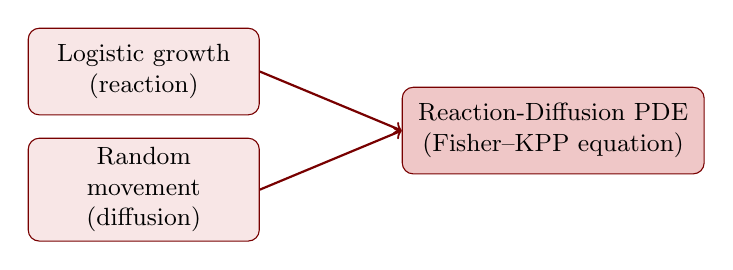
\begin{tikzpicture}[
            box/.style={draw=myNewColorA, fill=myNewColorC!20, rounded corners,
                        align=center, minimum height=1.1cm, text width=2.7cm, font=\small},
            arr/.style={->, thick, myNewColorA}]
          \node[box] (growth) at (0, 0.75)  {Logistic growth\\(reaction)};
          \node[box] (move)   at (0, -0.75) {Random movement\\(diffusion)};
          \node[box, text width=3.6cm, fill=myNewColorC!45] (pde) at (5.2, 0)
                {Reaction-Diffusion PDE\\(Fisher--KPP equation)};
          \draw[arr] (growth.east) -- (pde.west);
          \draw[arr] (move.east)   -- (pde.west);
        \end{tikzpicture}
      \end{center}
      \begin{block}{Why this project?}
          Instead of studying ODEs and PDEs only from a theoretical perspective, we apply them to a concrete mathematical-biology problem: from deriving the model, to solving it numerically, to visualizing how the population spreads.
      \end{block}
    \end{frame}

\section{Research Objectives}
    \begin{frame}{2. Research Objectives}
      \begin{block}{Goal}
          Simulate how a population \textbf{grows} and \textbf{spreads} in space.
      \end{block}
      \vspace{0.3cm}
      \begin{center}
        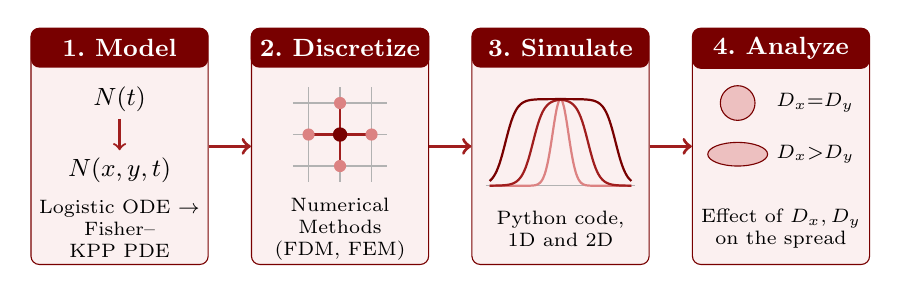
\begin{tikzpicture}[
            card/.style={draw=myNewColorA, fill=myNewColorC!12, rounded corners=3pt,
                         minimum width=2.25cm, minimum height=3cm},
            head/.style={fill=myNewColorA, text=white, rounded corners=3pt,
                         minimum width=2.25cm, minimum height=0.5cm, font=\small\bfseries},
            note/.style={font=\scriptsize, align=center, text width=2.1cm},
            flow/.style={->, very thick, myNewColorB}]
          % four steps
          \foreach \i/\n/\name in {0/1/Model, 1/2/Discretize, 2/3/Simulate, 3/4/Analyze} {
            \node[card] (c\i) at (2.8*\i, 0) {};
            \node[head, anchor=north] at (c\i.north) {\n.\ \name};
          }
          \foreach \i/\j in {0/1, 1/2, 2/3}
            \draw[flow] (c\i.east) -- (c\j.west);

          % 1. Model: from N(t) to N(x,y,t)
          \node[font=\small] at (0, 0.6) {$N(t)$};
          \draw[->, thick, myNewColorB] (0, 0.35) -- (0, -0.05);
          \node[font=\small] at (0, -0.3) {$N(x,y,t)$};
          \node[note] at (0, -1.05) {Logistic ODE $\to$\\ Fisher--KPP PDE};

          % 2. Discretize: five-point stencil
          \begin{scope}[shift={(2.8, 0.15)}]
            \draw[step=0.4, gray!60] (-0.6, -0.6) grid (0.6, 0.6);
            \draw[thick, myNewColorB] (-0.4, 0) -- (0.4, 0) (0, -0.4) -- (0, 0.4);
            \foreach \p in {(-0.4,0), (0.4,0), (0,-0.4), (0,0.4)}
              \fill[myNewColorC] \p circle (2.2pt);
            \fill[myNewColorA] (0, 0) circle (2.6pt);
          \end{scope}
          \node[note] at (2.8, -1.05) {Numerical Methods\\(FDM, FEM)};

          % 3. Simulate: a 1D front spreading out over time
          \begin{scope}[shift={(5.6, -0.5)}]
            \draw[gray!60] (-0.95, 0) -- (0.95, 0);
            \draw[thick, myNewColorC] plot[domain=-0.9:0.9, samples=60, smooth]
              (\x, {1.1*exp(-\x*\x/0.02)});
            \draw[thick, myNewColorB] plot[domain=-0.9:0.9, samples=60, smooth]
              (\x, {1.1/(1 + exp((abs(\x) - 0.35)/0.07))});
            \draw[thick, myNewColorA] plot[domain=-0.9:0.9, samples=60, smooth]
              (\x, {1.1/(1 + exp((abs(\x) - 0.7)/0.07))});
          \end{scope}
          \node[note] at (5.6, -1.05) {Python code,\\ 1D and 2D};

          % 4. Analyze: isotropic vs anisotropic spreading
          \begin{scope}[shift={(8.4, 0.15)}]
            \filldraw[fill=myNewColorC!50, draw=myNewColorA] (-0.55, 0.4) circle (0.22);
            \filldraw[fill=myNewColorC!50, draw=myNewColorA] (-0.55, -0.25) ellipse (0.38 and 0.15);
            \node[font=\scriptsize, anchor=west, inner sep=1pt] at (-0.1, 0.4) {$D_x{=}D_y$};
            \node[font=\scriptsize, anchor=west, inner sep=1pt] at (-0.1, -0.25) {$D_x{>}D_y$};
          \end{scope}
          \node[note] at (8.4, -1.05) {Effect of $D_x, D_y$\\ on the spread};
        \end{tikzpicture}
      \end{center}
    \end{frame}

\section{Literature Review}
  \subsection{Previous Studies}
    \begin{frame}{3. Literature Review}{Historical Background}
      \begin{block}{The Fisher--KPP equation}
          \begin{itemize}
              \item \textbf{1937:} Fisher [2] proposed the equation to describe the spread of an advantageous gene through a population. In the same year, Kolmogorov, Petrovskii and Piskunov [3] studied it rigorously.
              \item Main result: the equation has \textbf{traveling wave} solutions, i.e.\ a front that moves at the constant speed
              $$
              c^{*} = 2\sqrt{rD}.
              $$
              \item \textbf{1951:} Skellam [5] first applied the model to a real population: muskrats spreading across Central Europe after 1905. The square root of the occupied area grew linearly in time, as the model predicts.
          \end{itemize}
      \end{block}
    \end{frame}

    \begin{frame}{3. Literature Review}{Applications in Practice}
      \begin{center}
        \small
        \renewcommand{\arraystretch}{1.3}
        \begin{tabular}{l l c}
          \hline
          \textbf{Field} & \textbf{Phenomenon} & \textbf{Ref.} \\
          \hline
          Ecology & Invasive species (muskrats, butterflies) & [5], [6] \\
          Epidemiology & Rabies spreading among foxes in Europe & [7] \\
          Medicine & Brain tumor (glioma) growth on MRI & [8] \\
          Archaeology & Spread of farming in Neolithic Europe ($\approx 1$ km/year) & [9] \\
          Experiment & Invasion fronts of microorganisms in the lab & [10] \\
          \hline
        \end{tabular}
      \end{center}
      \begin{block}{Common approach}
          Estimate $D$ and $r$ from data $\Rightarrow$ predict the spreading speed $c^{*} = 2\sqrt{rD}$ $\Rightarrow$ compare it with the observed spread.
      \end{block}
    \end{frame}

  \subsection{Mathematical Modeling}
    \begin{frame}{3. Literature Review}{Mathematical Modeling: When ODE and PDE Combine}
      \begin{center}
        \begin{block}{Exponential Population Growth Equation}
            \begin{minipage}{\textwidth}
              Firstly, we start with a simple Exponential Population Growth Equation as below:
              $$
              \dfrac{dN}{dt} = rN
              $$
              Where $N(t)$ is the population size at time $t$, and $r$ is the growth rate (can be a constant $r$ or a function over time $r(t)$; to be simple we assume that $r = const$).
            \end{minipage}
        \end{block}
      \end{center}
    \end{frame}

    \begin{frame}{3. Literature Review}{Mathematical Modeling: When ODE and PDE Combine}
      \begin{center}
        \begin{block}{Logistic Population Growth Equation}
            \begin{minipage}{\textwidth}
              Now that with the Carrying Capacity $K$, we can use a Logistic Model:
              $$
              \dfrac{dN}{dt} = r\Big(1 - \dfrac{N}{K}\Big)N
              $$
              \begin{itemize}
              \item $N \ll K$: The population grows exponentially.
              \item $N \rightarrow K$: The population's growth speed decreases.
              \item $N = K$: The population stops growing since $\dfrac{dN}{dt} = r\Big(1-\dfrac{N}{N}\Big)N = 0$.
              \end{itemize}
            \end{minipage}
        \end{block}
      \end{center}
    \end{frame}
    
    \begin{frame}{3. Literature Review}{Mathematical Modeling: When ODE and PDE Combine}
      \begin{center}
        \begin{block}{Reaction-Diffusion Equation}
            \begin{minipage}{\textwidth}
              Supposing that the population starts at the center of a fixed segment on the $Ox$ axis and it gradually spreads. The population density at the point $x$ at time $t$ is described by $N = N(x,t)$:
              $$
              \dfrac{\partial N}{\partial t} = \underbrace{D\dfrac{\partial^2 N}{\partial x^2}}_{\text{Diffusion}} + \underbrace{r\Big(1-\dfrac{N}{K}\Big)N}_{\text{Population Growth}}
              $$
              By normalizing the population density as $u = N/K$, the equation becomes the \textit{Fisher--KPP equation}.
              $$
              \dfrac{\partial u}{\partial t} = D\dfrac{\partial^2 u}{\partial x^2} + ru\Big(1-u\Big)
              $$
              Where $D > 0$ is the diffusion coefficient, which represents the rate at which the population spreads through space.
            \end{minipage}
        \end{block}
      \end{center}
    \end{frame}

    \begin{frame}{3. Literature Review}{Mathematical Modeling: Two-Dimensional Space}
      \begin{center}
        \begin{block}{Reaction-Diffusion Equation on Two-Dimensional Space}
            \begin{minipage}{\textwidth}
              Suppose that a population is initially concentrated at the center of a rectangular domain in the $Oxy$ plane and gradually spreads in both the horizontal and vertical directions. The population density at position $(x,y)$ and time $t$ is described by $N = N(x,y,t)$:
              $$
              \dfrac{\partial N}{\partial t} = D_x\dfrac{\partial^2 N}{\partial x^2} + D_y\dfrac{\partial^2 N}{\partial y^2} + r\Big(1-\dfrac{N}{K}\Big)N
              $$
              Where $D_x, D_y > 0$ are the diffusion coefficients representing the rates at which the population spreads in the horizontal and vertical directions, respectively.
            \end{minipage}
        \end{block}
      \end{center}
    \end{frame}

    \begin{frame}{3. Literature Review}{Mathematical Modeling: Two-Dimensional Space}
      \begin{center}
        \begin{block}{Reaction-Diffusion Equation on Two-Dimensional Space}
            \begin{minipage}{\textwidth}
              If $D_x = D_y$ then we can write in short as:
              $$
              \dfrac{\partial N}{\partial t} = D\Big(\dfrac{\partial^2 N}{\partial x^2} + \dfrac{\partial^2 N}{\partial y^2}\Big) + r\Big(1-\dfrac{N}{K}\Big)N
              $$
              Or even shorter:
              $$
              \dfrac{\partial N}{\partial t} = D \nabla^2 N + r\Big(1-\dfrac{N}{K}\Big)N
              $$
              Note that $D_x$, $D_y$, and $D$ may be functions of space and time, such as $D_x(x,y,t)$, $D_y(x,y,t)$, and $D(x,y,t)$. However, for simplicity, we assume that they are constants.
            \end{minipage}
        \end{block}
      \end{center}
    \end{frame}
    \begin{frame}{3. Literature Review}{Mathematical Modeling: Neumann Boundary Condition}
      \begin{block}{No-Flux Boundary Condition}
          We assume that the population cannot leave the domain. Therefore, there is no population flux across the boundary:
          $$
          \frac{\partial N}{\partial n}=0
          \qquad \text{on } \partial\Omega
          $$
          where $\partial\Omega$ denotes the boundary of the spatial domain.
      \end{block}
      \begin{block}{For a Rectangular Domain}
          For $\Omega=[0,L_x]\times[0,L_y]$, the Neumann Boundary Condition is:
          $$
          \begin{aligned}
          \frac{\partial N}{\partial x}(0,y,t)
          &=
          \frac{\partial N}{\partial x}(L_x,y,t)=0,\\[4pt]
          \frac{\partial N}{\partial y}(x,0,t)
          &=
          \frac{\partial N}{\partial y}(x,L_y,t)=0.
          \end{aligned}
          $$
      \end{block}
    \end{frame}

    \begin{frame}{3. Literature Review}{Mathematical Modeling: Dirichlet Boundary Condition}
      \begin{block}{Dirichlet Boundary Condition}
          Instead of specifying the population flux, we specify the population density directly on the boundary:
          $$
          N(x,y,t)=g(x,y,t)
          \qquad \text{on } \partial\Omega.
          $$
          For example, a zero-density boundary condition is:
          $$
          N(x,y,t)=0
          \qquad \text{on } \partial\Omega.
          $$
      \end{block}
      \begin{block}{Interpretation}
          The population density is prescribed at the boundary.

          Unlike the Neumann condition, individuals may cross the boundary.

          To be simple we use Neumann Boundary Condition in this presentation.
      \end{block}
    \end{frame}

\section{Research Methodology}
  \subsection{Finite Difference Method}
    \begin{frame}{4. Research Methodology}{Spatial Discretization}
      \begin{columns}[c]
        \begin{column}{0.5\textwidth}
          \begin{block}{Finite Difference Method}
              We discretize the spatial domain into a uniform grid:
              $$
              x_i=i\Delta x,\qquad
              y_j=j\Delta y
              $$
              and approximate the population density by
              $$
              N(x_i,y_j,t)\approx N_{i,j}(t).
              $$
          \end{block}
        \end{column}
        \begin{column}{0.45\textwidth}
          \begin{center}
            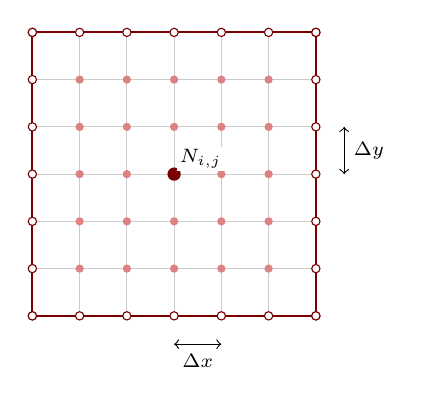
\begin{tikzpicture}[scale=0.6]
              \draw[gray!40] (0,0) grid (6,6);
              \draw[myNewColorA, thick] (0,0) rectangle (6,6);
              \foreach \i in {1,...,5}
                \foreach \j in {1,...,5}
                  \fill[myNewColorC] (\i,\j) circle (2.5pt);
              \foreach \k in {0,...,6} {
                \filldraw[fill=white, draw=myNewColorA] (\k,0) circle (2.5pt);
                \filldraw[fill=white, draw=myNewColorA] (\k,6) circle (2.5pt);
                \filldraw[fill=white, draw=myNewColorA] (0,\k) circle (2.5pt);
                \filldraw[fill=white, draw=myNewColorA] (6,\k) circle (2.5pt);
              }
              \fill[myNewColorA] (3,3) circle (4pt);
              \node[above right, font=\scriptsize, fill=white, inner sep=1pt] at (3.05,3.05) {$N_{i,j}$};
              \draw[<->] (3,-0.6) -- (4,-0.6) node[midway, below, font=\scriptsize] {$\Delta x$};
              \draw[<->] (6.6,3) -- (6.6,4) node[midway, right, font=\scriptsize] {$\Delta y$};
            \end{tikzpicture}

            {\scriptsize
            \tikz\fill[myNewColorC] (0,0) circle (2.5pt); interior node \quad
            \tikz\filldraw[fill=white, draw=myNewColorA] (0,0) circle (2.5pt); boundary node}
          \end{center}
        \end{column}
      \end{columns}
    \end{frame}

    \begin{frame}{4. Research Methodology}{Second-Order Spatial Derivatives}
      \begin{block}{Second-Order Spatial Derivatives}
          Using the central difference approximation $$f''(x) \approx \dfrac{f(x+h) - 2f(x) + f(x-h)}{h^2}$$
          Then:
          $$
          N_{xx} = \frac{\partial^2N}{\partial x^2}
          \approx
          \frac{N_{i+1,j}-2N_{i,j}+N_{i-1,j}}
          {(\Delta x)^2}
          $$
          $$
          N_{yy} = \frac{\partial^2N}{\partial y^2}
          \approx
          \frac{N_{i,j+1}-2N_{i,j}+N_{i,j-1}}
          {(\Delta y)^2}.
          $$
      \end{block}
    \end{frame}
    \begin{frame}{4. Research Methodology}{Time Discretization}
      Let
      $$
      t_n=n\Delta t,
      \qquad
      N_{i,j}^n\approx N(x_i,y_j,t_n).
      $$
      Using the Explicit Euler method:
      $$
      \frac{\partial N}{\partial t}
      \approx
      \frac{N_{i,j}^{n+1}-N_{i,j}^{n}}
      {\Delta t}.
      $$
      Therefore,
      $$
      N_{i,j}^{n+1}
      =
      N_{i,j}^{n}
      +
      \Delta t \Big[D_x N_{xx} + D_y N_{yy} + rN^n_{i, j} \Big(1 - \dfrac{N^n_{i, j}}{K} \Big)\Big].
      $$
    \end{frame}

  \subsection{Boundary Condition and Stability}
    \begin{frame}{4. Research Methodology}{Discrete Boundary Condition}
      \begin{columns}[c]
        \begin{column}{0.55\textwidth}
          \begin{block}{Neumann condition on the grid}
              At the left edge, replace $\dfrac{\partial N}{\partial x} = 0$ by a one-sided difference:
              $$
              \frac{N_{1,j} - N_{0,j}}{\Delta x} = 0
              \;\Longrightarrow\;
              N_{0,j} = N_{1,j}.
              $$
          \end{block}
        \end{column}
        \begin{column}{0.4\textwidth}
          \begin{center}
            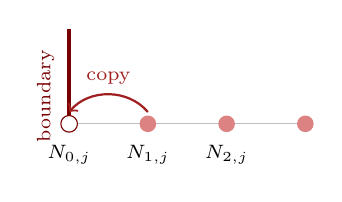
\begin{tikzpicture}
              \draw[myNewColorA, very thick] (0,0) -- (0,1.2);
              \node[font=\scriptsize, myNewColorA, rotate=90] at (-0.3,0.35) {boundary};
              \draw[gray!50] (0,0) -- (3,0);
              \filldraw[fill=white, draw=myNewColorA] (0,0) circle (3pt);
              \foreach \k in {1,2,3}
                \fill[myNewColorC] (\k,0) circle (3pt);
              \node[below, font=\scriptsize] at (0,-0.15) {$N_{0,j}$};
              \node[below, font=\scriptsize] at (1,-0.15) {$N_{1,j}$};
              \node[below, font=\scriptsize] at (2,-0.15) {$N_{2,j}$};
              \draw[->, thick, myNewColorB] (1,0.15) to[bend right=50]
                    node[above, font=\scriptsize] {copy} (0,0.15);
            \end{tikzpicture}
          \end{center}
        \end{column}
      \end{columns}
      \vspace{0.3cm}
      \begin{block}{After every time step, each boundary node copies its inner neighbor}
          $$
          N_{0,j} = N_{1,j},\qquad
          N_{N_x,j} = N_{N_x-1,j},\qquad
          N_{i,0} = N_{i,1},\qquad
          N_{i,N_y} = N_{i,N_y-1}.
          $$
      \end{block}
    \end{frame}

    \begin{frame}{4. Research Methodology}{Stability Condition}
      \begin{block}{Courant - Friedrichs - Lewy (CFL) Stability Condition \hfill [4]}
          $$
          \Delta t \;\le\; \Delta t_{\max} = \frac{1}{2\Big(\dfrac{D_x}{\Delta x^2} + \dfrac{D_y}{\Delta y^2}\Big)}
          \qquad
          \Big(\text{1D: } \Delta t \le \frac{\Delta x^2}{2D}\Big)
          $$
      \end{block}
      \begin{center}
        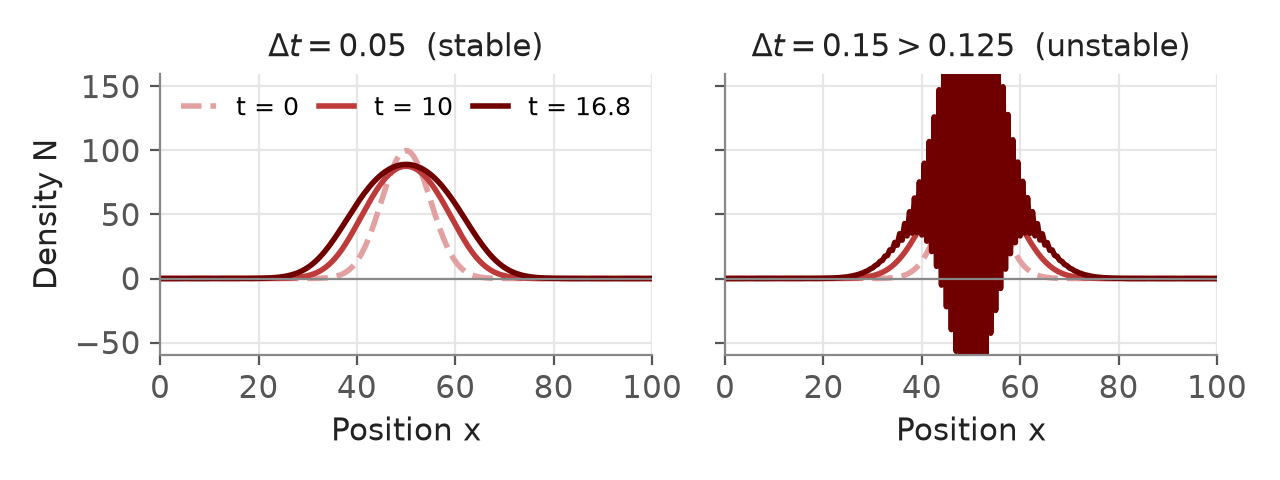
\includegraphics[width=\textwidth]{./Fig4_stability.png}
      \end{center}
    \end{frame}

  \subsection{Finite Element Method}
    \begin{frame}{4. Research Methodology}{Finite Element Method: Weak Formulation}
      \begin{block}{Weak form \hfill [11]}
          Multiply the PDE by a test function $v$, integrate over $\Omega$ and integrate by parts ($f(N) = rN(1 - N/K)$):
          $$
          \begin{aligned}
          \int_\Omega N_t\, v \, d\mathbf{x}
          + \int_\Omega \big(D_x N_x v_x + D_y N_y v_y\big)\, d\mathbf{x}
          &= \int_\Omega f(N)\, v \, d\mathbf{x} \\
          &\quad + \underbrace{\oint_{\partial\Omega} v\,\big(D_x N_x n_x + D_y N_y n_y\big)\, ds}_{=\,0 \text{ by the no-flux condition}}
          \end{aligned}
          $$
      \end{block}
      \begin{alertblock}{Natural boundary condition}
          The Neumann condition removes the boundary term: nothing has to be imposed at the boundary.
      \end{alertblock}
    \end{frame}

    \begin{frame}{4. Research Methodology}{Finite Element Method: Galerkin Discretization}
      \begin{columns}[c]
        \begin{column}{0.42\textwidth}
          \begin{center}
            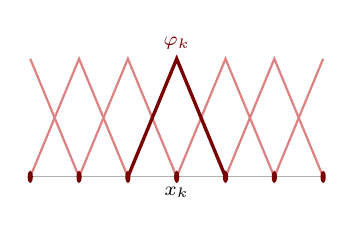
\begin{tikzpicture}[xscale=0.62, yscale=1.5]
              \draw[gray!60] (0,0) -- (6,0);
              \foreach \k in {1,...,5}
                \draw[myNewColorC, thick] (\k-1,0) -- (\k,1) -- (\k+1,0);
              \draw[myNewColorC, thick] (0,1) -- (1,0);
              \draw[myNewColorC, thick] (5,0) -- (6,1);
              \draw[myNewColorA, very thick] (2,0) -- (3,1) -- (4,0);
              \node[above, font=\scriptsize, myNewColorA] at (3,1) {$\varphi_k$};
              \foreach \k in {0,...,6}
                \fill[myNewColorA] (\k,0) circle (1.5pt);
              \node[below, font=\scriptsize] at (3,0) {$x_k$};
            \end{tikzpicture}

            {\scriptsize $\varphi_k = 1$ at $x_k$, $0$ at other nodes}
          \end{center}
        \end{column}
        \begin{column}{0.56\textwidth}
          \begin{block}{Approximation}
              $$
              N(\mathbf{x},t) \approx \sum_k N_k(t)\, \varphi_k(\mathbf{x})
              $$
              In 2D: bilinear elements $\varphi_i(x)\,\psi_j(y)$ on the same grid as the FDM.
          \end{block}
        \end{column}
      \end{columns}
      \begin{block}{Choosing $v = \varphi_l$ gives a system of ODEs}
          $$
          M\,\frac{d\mathbf{N}}{dt} + S\,\mathbf{N} = M f(\mathbf{N})
          $$
          $$
          \underbrace{M_{kl} = \int_\Omega \varphi_k\varphi_l}_{\text{mass matrix}},
          \qquad
          \underbrace{S_{kl} = \int_\Omega \big(D_x\, \partial_x\varphi_k\, \partial_x\varphi_l + D_y\, \partial_y\varphi_k\, \partial_y\varphi_l\big)}_{\text{stiffness matrix}}
          $$
      \end{block}
    \end{frame}

    \begin{frame}{4. Research Methodology}{Finite Element Method: Time Stepping}
      \begin{block}{Semi-implicit Euler: diffusion implicit, reaction explicit}
          $$
          (M + \Delta t\, S)\,\mathbf{N}^{n+1} = M\big(\mathbf{N}^{n} + \Delta t\, f(\mathbf{N}^{n})\big)
          $$
          No stability limit from diffusion $\Rightarrow$ we can use $\Delta t = 0.5$.
      \end{block}
      \begin{center}
        \small
        \renewcommand{\arraystretch}{1.3}
        \begin{tabular}{l l l}
          \hline
          & \textbf{FDM} & \textbf{FEM} \\
          \hline
          Unknowns & values $N_{i,j}$ at grid points & coefficients of $\varphi_k$ \\
          Neumann condition & copy the inner neighbor & natural (automatic) \\
          Time step & explicit, $\Delta t \le \Delta t_{\max}$ & semi-implicit, larger $\Delta t$ \\
          Cost per step & cheap update & one linear solve \\
          Domain & rectangular grid & any shape (triangular mesh) \\
          \hline
        \end{tabular}
      \end{center}
    \end{frame}

  \subsection{ADI Method}
    \begin{frame}{4. Research Methodology}{ADI Method: Alternating Directions}
      \begin{block}{Peaceman--Rachford ADI \hfill [4], [12]}
          Each step is split into two half steps, each implicit in \textbf{one} direction only:
          $$
          \begin{aligned}
          \Big(I - \tfrac{\Delta t}{2} D_x L_x\Big) N^{*} &= \Big(I + \tfrac{\Delta t}{2} D_y L_y\Big) N^{n} & &\text{implicit in } x \\
          \Big(I - \tfrac{\Delta t}{2} D_y L_y\Big) N^{n+1} &= \Big(I + \tfrac{\Delta t}{2} D_x L_x\Big) N^{*} & &\text{implicit in } y
          \end{aligned}
          $$
          {\small $L_x, L_y$: central second differences; Neumann condition through a ghost point $N_{-1,j} = N_{1,j}$.}
      \end{block}
      \begin{center}
        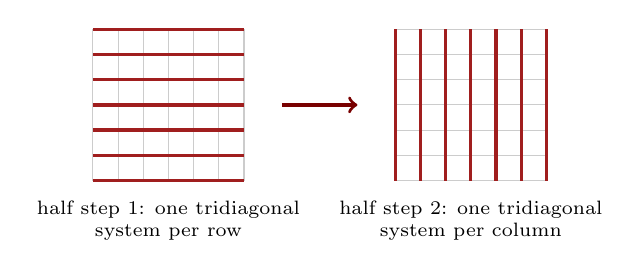
\begin{tikzpicture}[scale=0.32]
          % half step 1: rows
          \draw[gray!40] (0,0) grid (6,6);
          \foreach \j in {0,...,6}
            \draw[myNewColorB, very thick] (0,\j) -- (6,\j);
          \node[font=\scriptsize, align=center] at (3,-1.6) {half step 1: one tridiagonal\\system per row};
          \draw[->, very thick, myNewColorA] (7.5,3) -- (10.5,3);
          % half step 2: columns
          \begin{scope}[shift={(12,0)}]
            \draw[gray!40] (0,0) grid (6,6);
            \foreach \i in {0,...,6}
              \draw[myNewColorB, very thick] (\i,0) -- (\i,6);
            \node[font=\scriptsize, align=center] at (3,-1.6) {half step 2: one tridiagonal\\system per column};
          \end{scope}
        \end{tikzpicture}
      \end{center}
    \end{frame}

    \begin{frame}{4. Research Methodology}{ADI Method: Treating the Logistic Term}
      \begin{block}{Strang splitting of one time step \hfill [13]}
          \begin{center}
            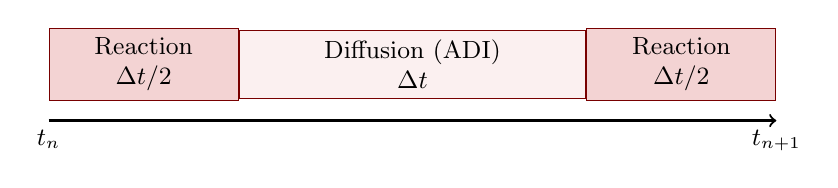
\begin{tikzpicture}[
                part/.style={draw=myNewColorA, minimum height=0.8cm, font=\small, align=center}]
              \node[part, fill=myNewColorC!35, minimum width=2.4cm] (r1) at (0,0)   {Reaction\\$\Delta t/2$};
              \node[part, fill=myNewColorC!12, minimum width=4.4cm, anchor=west] (d) at (r1.east) {Diffusion (ADI)\\$\Delta t$};
              \node[part, fill=myNewColorC!35, minimum width=2.4cm, anchor=west] (r2) at (d.east) {Reaction\\$\Delta t/2$};
              \draw[->, thick] ([yshift=-0.25cm]r1.south west) -- ([yshift=-0.25cm]r2.south east);
              \node[below, font=\small] at ([yshift=-0.25cm]r1.south west) {$t_n$};
              \node[below, font=\small] at ([yshift=-0.25cm]r2.south east) {$t_{n+1}$};
            \end{tikzpicture}
          \end{center}
      \end{block}
      \begin{block}{The reaction part has an exact solution (logistic ODE)}
          $$
          N(t) = \frac{K N_0\, e^{rt}}{K + N_0\big(e^{rt} - 1\big)}
          $$
      \end{block}
      \begin{alertblock}{Result}
          Unconditionally stable and second-order accurate in time: $\Delta t$ is limited by accuracy only.
      \end{alertblock}
    \end{frame}

  \subsection{Implementation}
    \begin{frame}{4. Research Methodology}{Implementation}
      \begin{columns}[c]
        \begin{column}{0.48\textwidth}
          \begin{center}
            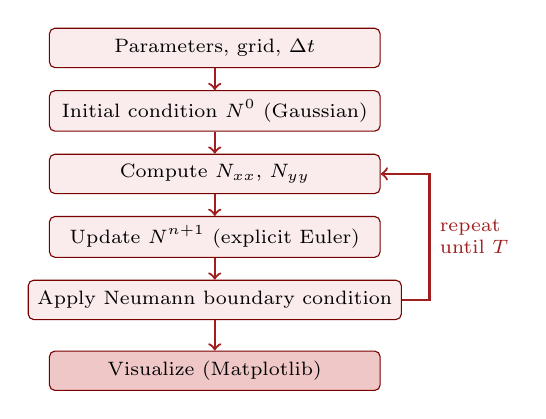
\begin{tikzpicture}[
                stage/.style={draw=myNewColorA, fill=myNewColorC!15, rounded corners=2pt,
                              minimum width=4.2cm, minimum height=0.5cm, font=\scriptsize},
                go/.style={->, thick, myNewColorB}]
              \node[stage] (s1) at (0, 0)    {Parameters, grid, $\Delta t$};
              \node[stage] (s2) at (0,-0.8)  {Initial condition $N^0$ (Gaussian)};
              \node[stage] (s3) at (0,-1.6)  {Compute $N_{xx}$, $N_{yy}$};
              \node[stage] (s4) at (0,-2.4)  {Update $N^{n+1}$ (explicit Euler)};
              \node[stage] (s5) at (0,-3.2)  {Apply Neumann boundary condition};
              \node[stage, fill=myNewColorC!45] (s6) at (0,-4.1) {Visualize (Matplotlib)};
              \foreach \a/\b in {s1/s2, s2/s3, s3/s4, s4/s5, s5/s6}
                \draw[go] (\a) -- (\b);
              \draw[go] (s5.east) -- ++(0.35,0) |- (s3.east)
                    node[pos=0.25, right, font=\scriptsize, align=left] {repeat\\until $T$};
            \end{tikzpicture}

            {\scriptsize FEM: loop body = one linear solve}
          \end{center}
        \end{column}
        \begin{column}{0.48\textwidth}
          \begin{block}{Numerical settings}
              \centering
              \small
              \renewcommand{\arraystretch}{1.3}
              \begin{tabular}{l c c}
                  & \textbf{1D} & \textbf{2D} \\
                  \hline
                  $\Delta x \; (= \Delta y)$ & $0.5$ & $1$ \\
                  $\Delta t_{\max}$ (FDM) & $0.125$ & $0.1$ \\
                  $\Delta t$ FDM & $0.05$ & $0.08$ \\
                  $\Delta t$ FEM & $0.5$ & $0.5$ \\
              \end{tabular}
          \end{block}
          \begin{block}{Tools}
              Python, NumPy (vectorized arrays), Matplotlib
          \end{block}
        \end{column}
      \end{columns}
    \end{frame}

\section{Results and Discussion}
  \subsection{One-Dimensional Simulation}
    \begin{frame}{5. Results and Discussion}{One-Dimensional Simulation}
      Suppose we have a population of animals in a closed one-dimensional habitat
      $$
      \Omega = [0,100]
      $$
      and no animal can cross the boundary of the domain. Therefore, the Neumann Boundary Condition is:
      $$
      \frac{\partial N}{\partial x}(0,t)
      =
      \frac{\partial N}{\partial x}(100,t)
      =
      0.
      $$
      We choose the simulation constants:
      $$
      D=1,\qquad r=0.1,\qquad K=100.
      $$
    \end{frame}
    \begin{frame}{5. Results and Discussion}{One-Dimensional Simulation}
      We choose the initial population distribution:
      $$
      N(x,0)
      =
      N_0
      \exp\left[
      -\frac{(x-x_0)^2}{2\sigma^2}
      \right].
      $$
      Suppose that the population initially concentrates at the center of the domain, where
      $$
      x_0=50,\qquad N_0=100,\qquad \sigma=5.
      $$
      Then the initial population distribution is:
      $$
      N(x,0)
      =
      100
      \exp\left[
      -\frac{(x-50)^2}{50}
      \right].
      $$
    \end{frame}
    \begin{frame}{5. Results and Discussion}{One-Dimensional Simulation}
      \begin{center}
        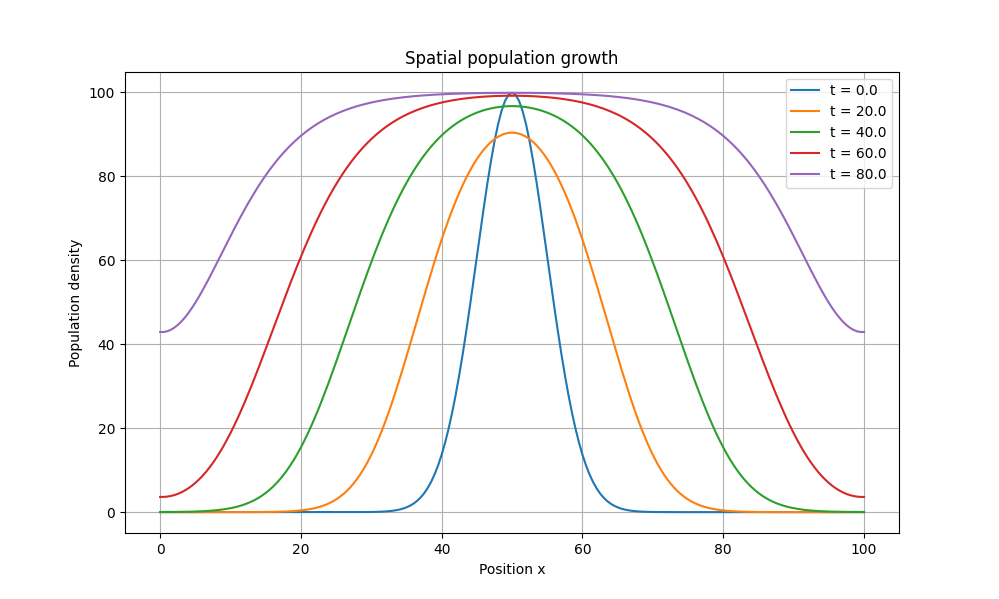
\includegraphics[height=6.5cm]{./Fig1.png}
      \end{center}
    \end{frame}
    \begin{frame}{5. Results and Discussion}{One-Dimensional Simulation}
      \begin{center}
        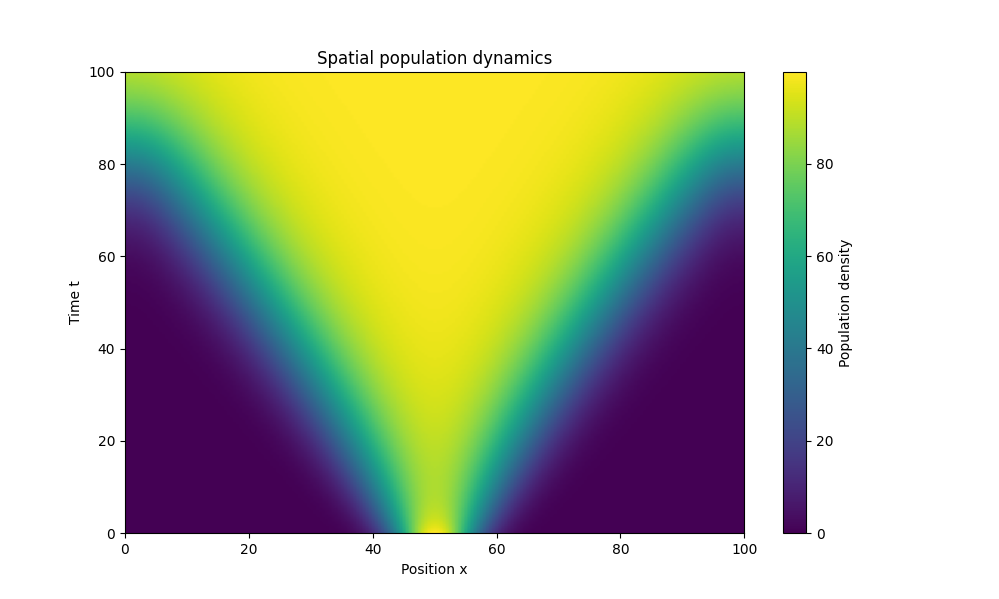
\includegraphics[height=6.5cm]{./Fig2.png}
      \end{center}
    \end{frame}

  \subsection{Two-Dimensional Simulation}
    \begin{frame}{5. Results and Discussion}{Two-Dimensional Simulation}
      Suppose we have a population of animals in a closed rectangular domain 
      $$\Omega = [0, 100] \times [0, 100]$$
      and no animals can leave the domain. So the Neumann Boundary Condition is:
      $$
            \begin{aligned}
            \frac{\partial N}{\partial x}(0,y,t)
            &=
            \frac{\partial N}{\partial x}(100,y,t)=0,\\[4pt]
            \frac{\partial N}{\partial y}(x,0,t)
            &=
            \frac{\partial N}{\partial y}(x,100,t)=0.
            \end{aligned}
            $$
      We choose simulation parameters:
      $$ D_x = 4, \qquad D_y = 1, \qquad r = 0.1, \qquad K = 100.$$
    \end{frame}

    \begin{frame}{5. Results and Discussion}{Two-Dimensional Simulation}
      And we choose the initial state:
      $$ N(x,y,0) = N_0 \exp \Big[-\dfrac{(x-x_0)^2 + (y-y_0)^2}{2\sigma^2}\Big]$$
      Suppose that the initial location is at the center of the rectangular domain $(x_0, y_0) = (50, 50)$, the maximum initial population density is $N_0 = 80$ and the initial population spread is $\sigma = 5$. Then we have:
      $$ N(x,y,0) = 80 \exp \Big[-\dfrac{(x-50)^2 + (y-50)^2}{50}\Big]$$
    \end{frame}

    \begin{frame}{5. Results and Discussion}{Two-Dimensional Simulation}
      \begin{center}
        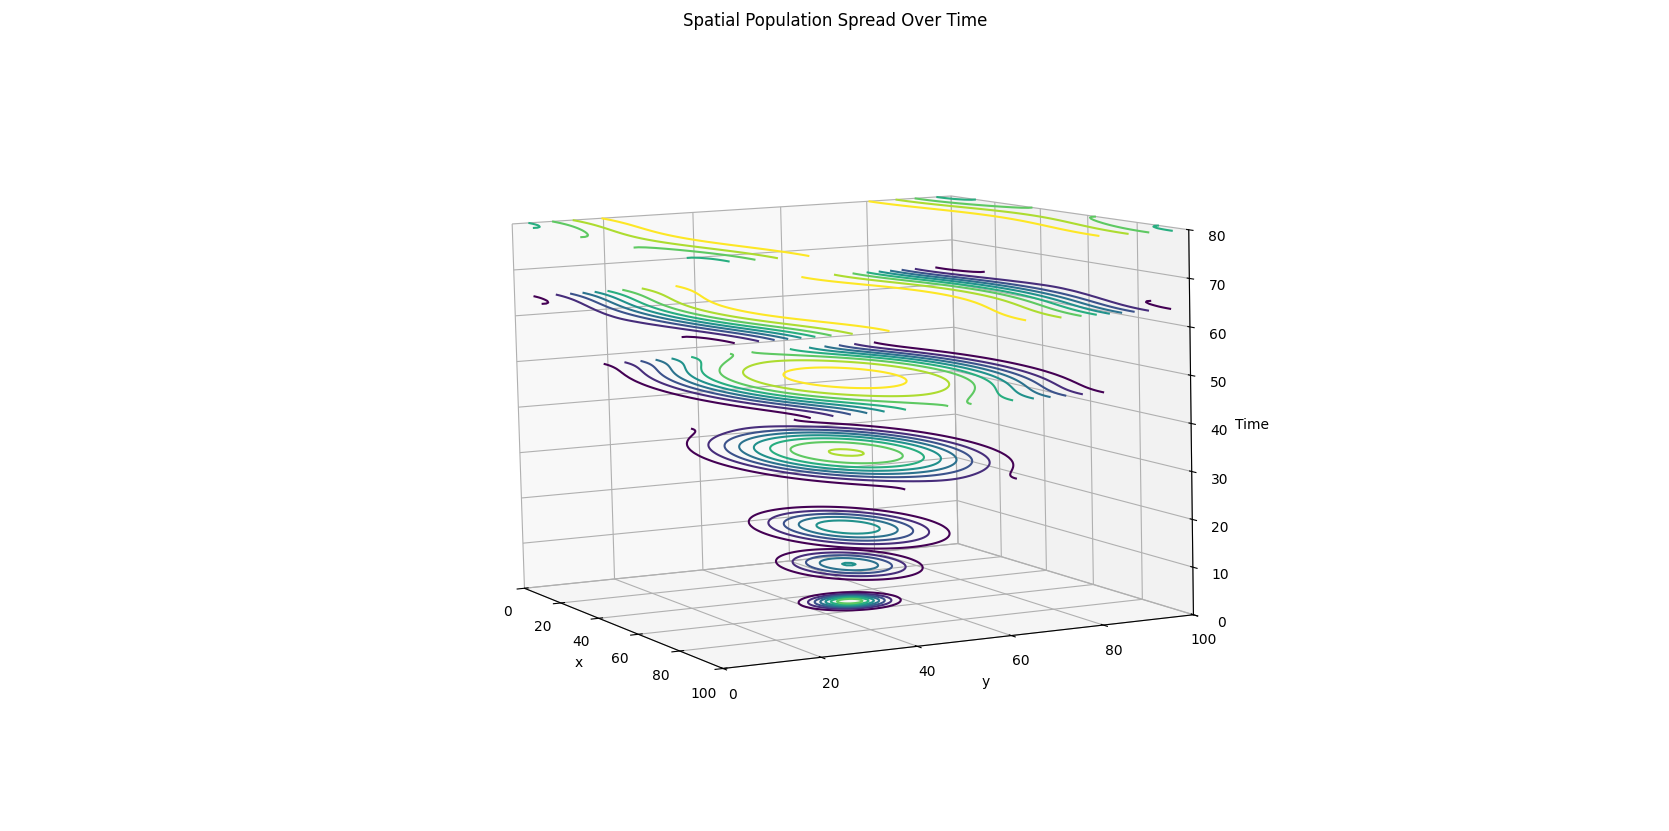
\includegraphics[height=6.5cm]{./Fig3.png}
      \end{center}
    \end{frame}

  \subsection{Real Terrain: Ba V\`{\i}}
    \begin{frame}{5. Results and Discussion}{Real Terrain (Ba V\`{\i}): Model and Terrain Functions}
      \begin{block}{Reaction--diffusion--taxis model}
          $$
          \frac{\partial N}{\partial t}
          = \underbrace{\nabla\cdot\big(D\,\nabla N\big)}_{\text{movement}}
          - \underbrace{\nabla\cdot\big(\chi\, N\, \nabla A\big)}_{\text{drift to good habitat}}
          + \underbrace{r\,N\Big(1-\frac{N}{K}\Big)}_{\text{local growth}}
          $$
          {\small $D, \chi, A, r, K$ depend on the position $\mathbf{x} = (x, y)$; no-flux boundary; $x, y$ in km, $t$ in years.}
      \end{block}
      \begin{block}{Terrain functions, built from the elevation $z(x,y)$}
          \centering
          \small
          \renewcommand{\arraystretch}{1.25}
          \begin{tabular}{l l l}
            Slope & $s = |\nabla z|$ & m per m \\
            Mobility & $D = D_0\, e^{-s/s_0}$ \quad (rivers: $\rho\, D_0$) & slow on slopes \\
            Carrying capacity & $K = K_0\, e^{-(z/z_c)^2}$ & poor high up \\
            Growth rate & $r = r_0$ \quad (rivers: $r_{\mathrm{riv}}$) & risky crossing \\
            Attraction & $A = K / K_0$ & good habitat \\
            Taxis & $\chi = \chi_0\, D / D_0$ & drift \\
          \end{tabular}
      \end{block}
    \end{frame}

    \begin{frame}{5. Results and Discussion}{Real Terrain (Ba V\`{\i}): Data, Grid and Initial Condition}
      \begin{block}{Data and grid}
          \small
          \renewcommand{\arraystretch}{1.25}
          \begin{tabular}{@{}p{2.4cm} p{7.7cm}@{}}
            \textbf{Elevation} & Copernicus DEM GLO-30 (30 m) \\
            \textbf{Rivers} & OpenStreetMap \\
            \textbf{Region} & $20.95$--$21.20^\circ$N, \; $105.20$--$105.55^\circ$E \quad ($36 \times 28$ km) \\
            \textbf{Grid} & $180 \times 252$ cells of $144 \times 154$ m (mean of $5 \times 5$ DEM pixels) \\
            \textbf{Time stepping} & finite volumes + explicit Euler, \; $\Delta t = 0.0043$ year, \; $6918$ steps to $T = 30$ years \\
          \end{tabular}
      \end{block}
      \begin{block}{Initial condition}
          \small
          \renewcommand{\arraystretch}{1.25}
          \begin{tabular}{@{}p{2.4cm} p{7.7cm}@{}}
            \textbf{Start} $\mathbf{x}_0$ & $21.10^\circ$N, $105.40^\circ$E: plain north-east of Ba V\`{\i}, \; $z = 43$ m \\
            \textbf{Density} & $N(\mathbf{x}, 0) = 80\, \exp\big(-|\mathbf{x} - \mathbf{x}_0|^2 / 2\sigma^2\big)$, \quad $\sigma = 0.5$ km \\
            \textbf{Arrival} & a cell counts as reached when $N \ge 0.2\,K_0 = 20$ \\
          \end{tabular}
      \end{block}
    \end{frame}

    \begin{frame}{5. Results and Discussion}{Real Terrain (Ba V\`{\i}): Constants}
      \begin{center}
        \small
        \renewcommand{\arraystretch}{1.15}
        \begin{tabular}{l l l}
          \hline
          \textbf{Constant} & \textbf{Value} & \textbf{Meaning} \\
          \hline
          $D_0$ & $1$ km$^2$/year & mobility on flat land \\
          $r_0$ & $0.5$ /year & growth rate on land \\
          $K_0$ & $100$ & carrying capacity in the lowland \\
          $\chi_0$ & $1$ km$^2$/year & strength of the drift \\
          $s_0$ & $0.2$ & slope scale (slope $0.6$: $D \approx 0.05\,D_0$) \\
          $z_c$ & $700$ m & altitude scale (summit: $K \approx 4$) \\
          $c = 2\sqrt{r_0 D_0}$ & $1.41$ km/year & Fisher--KPP front speed on flat land \\
          \hline
        \end{tabular}

        \vspace{0.3cm}
        \begin{tabular}{l c c c}
          \hline
          \textbf{River} & \textbf{Width on the grid} & $\rho = D/D_0$ & $r_{\mathrm{riv}}$ \\
          \hline
          Red River & $5$ cells $\approx 700$ m & $0.002$ & $-2$ /year \\
          Da River & $3$ cells $\approx 450$ m & $0.002$ & $-2$ /year \\
          Tich River & $1$ cell $\approx 150$ m & $0.1$ & $0$ \\
          other rivers & $1$ cell & $0.3$ & $0$ \\
          \hline
        \end{tabular}

        \vspace{0.2cm}
        {\scriptsize Values are illustrative, not fitted to a particular species.}
      \end{center}
    \end{frame}

    \begin{frame}{5. Results and Discussion}{Real Terrain (Ba V\`{\i}): Elevation and Mobility}
      \begin{center}
        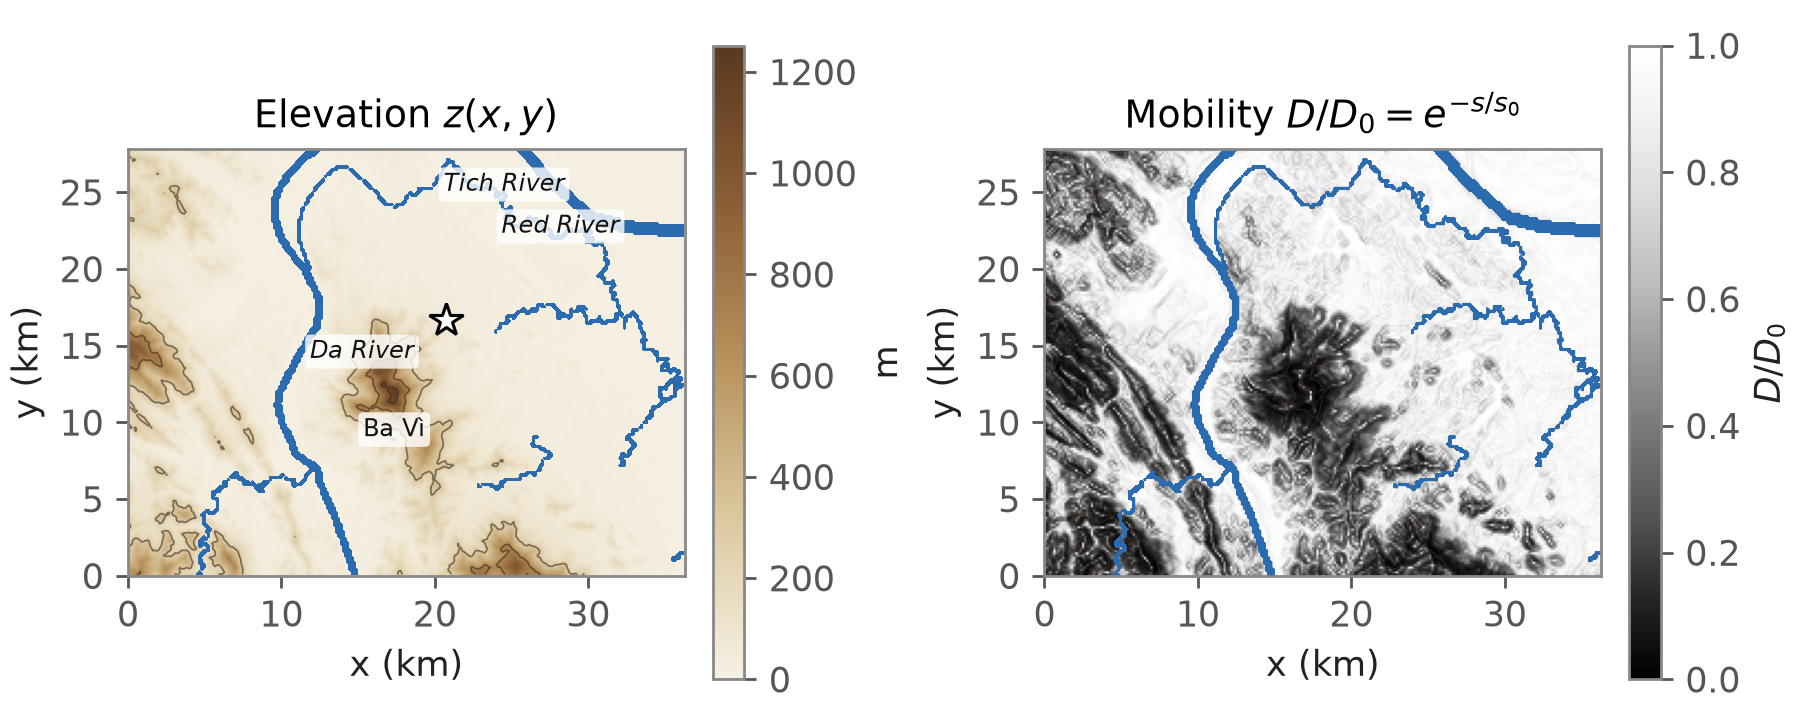
\includegraphics[width=\textwidth]{./FigB1a_bavi_elevation_mobility.png}
      \end{center}
      \begin{block}{Mobility $D = D_0\, e^{-s/s_0}$, \; $s = |\nabla z|$}
          Flat land: $D \approx D_0$. Steep flanks of Ba V\`{\i}: $D < 0.1\,D_0$. Rivers: $D = \rho\, D_0$ (blue).
      \end{block}
    \end{frame}

    \begin{frame}{5. Results and Discussion}{Real Terrain (Ba V\`{\i}): Habitat and Drift}
      \begin{center}
        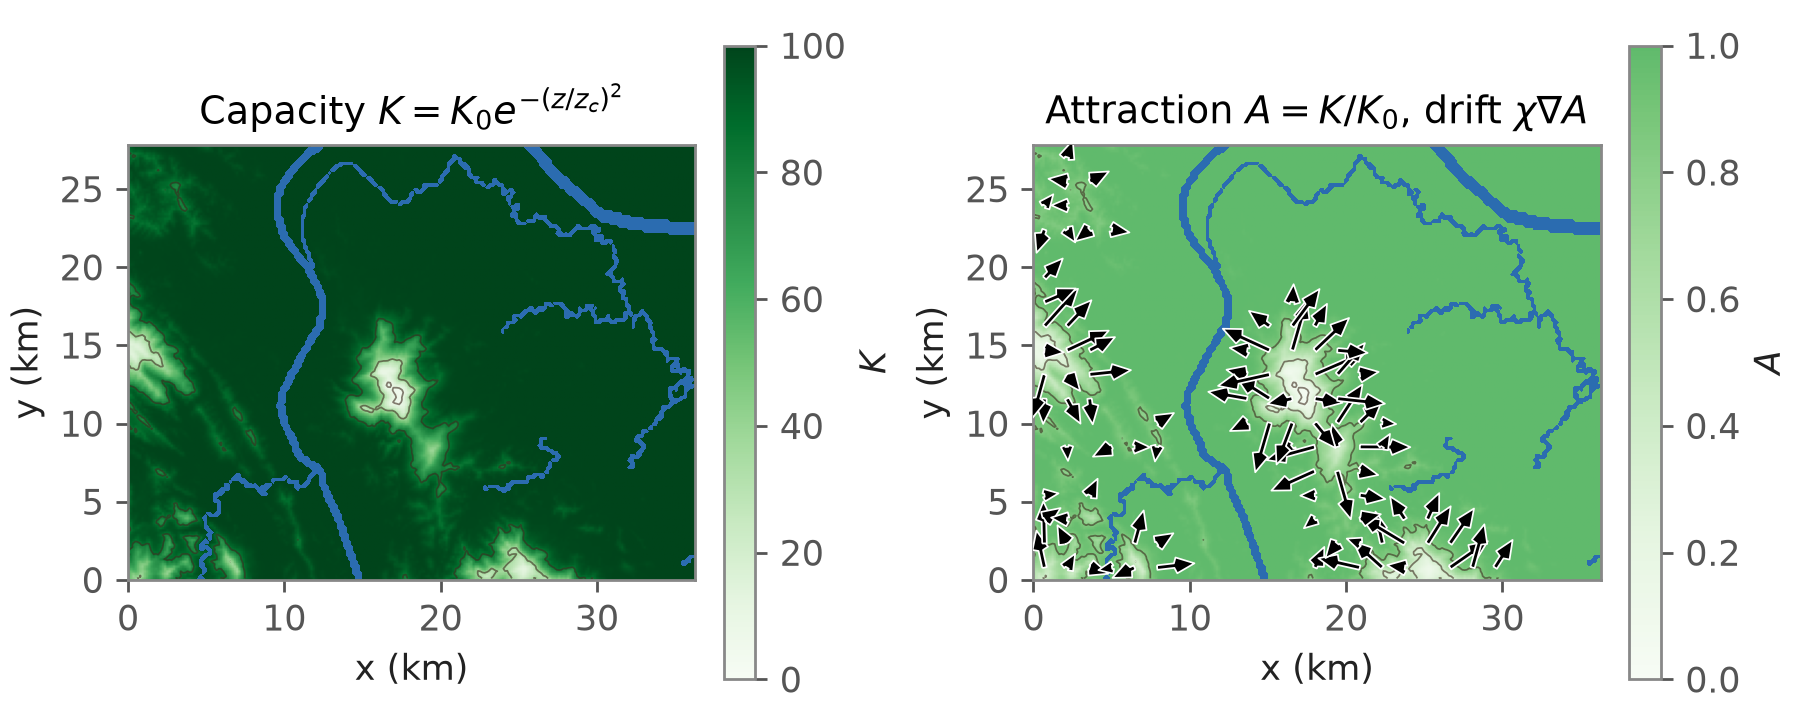
\includegraphics[width=\textwidth]{./FigB1b_bavi_capacity_attraction.png}
      \end{center}
      \begin{block}{Carrying capacity $K = K_0\, e^{-(z/z_c)^2}$}
          Lowland: $K \approx K_0 = 100$. Summit: $K \approx 4$. Arrows: drift $\chi \nabla A$ points downhill, toward better habitat.
      \end{block}
    \end{frame}

    \begin{frame}{5. Results and Discussion}{Real Terrain (Ba V\`{\i}): Population over 30 Years}
      \begin{center}
        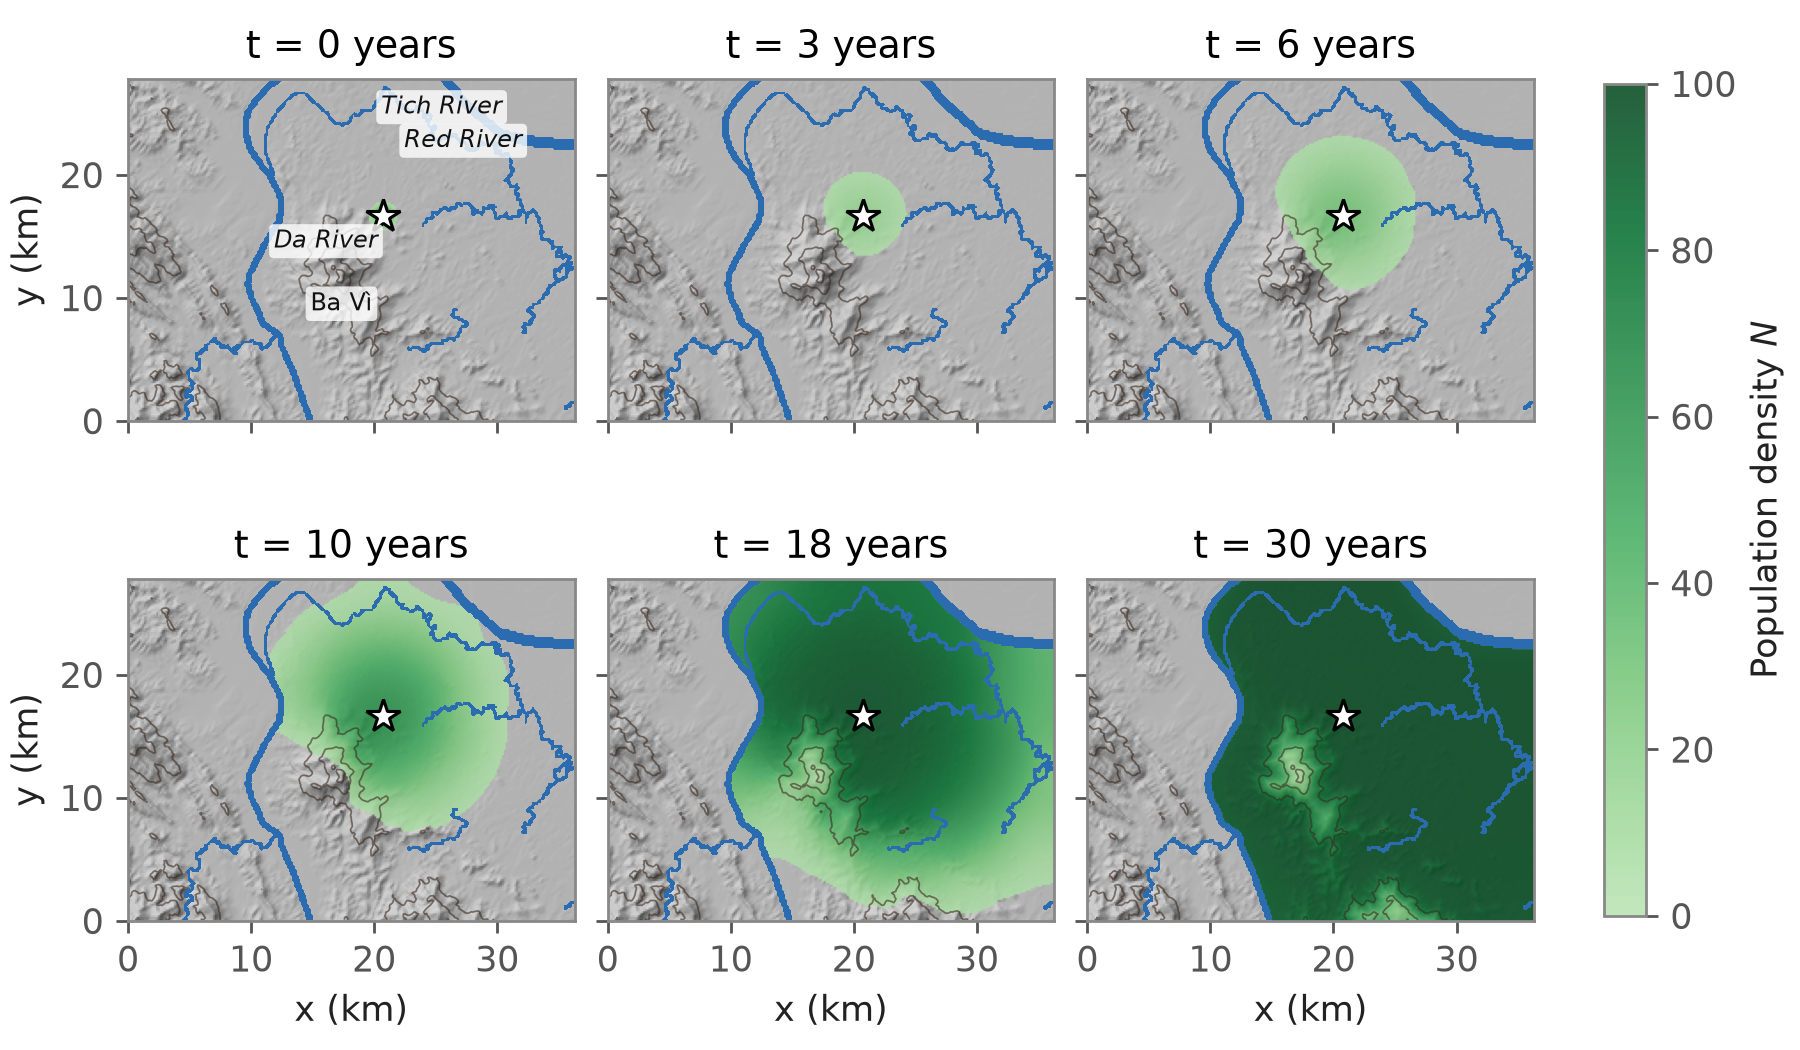
\includegraphics[height=6.4cm]{./FigB2_bavi_snapshots.png}
      \end{center}
    \end{frame}

    \begin{frame}{5. Results and Discussion}{Real Terrain (Ba V\`{\i}): Arrival Time and Front Speed}
      \begin{center}
        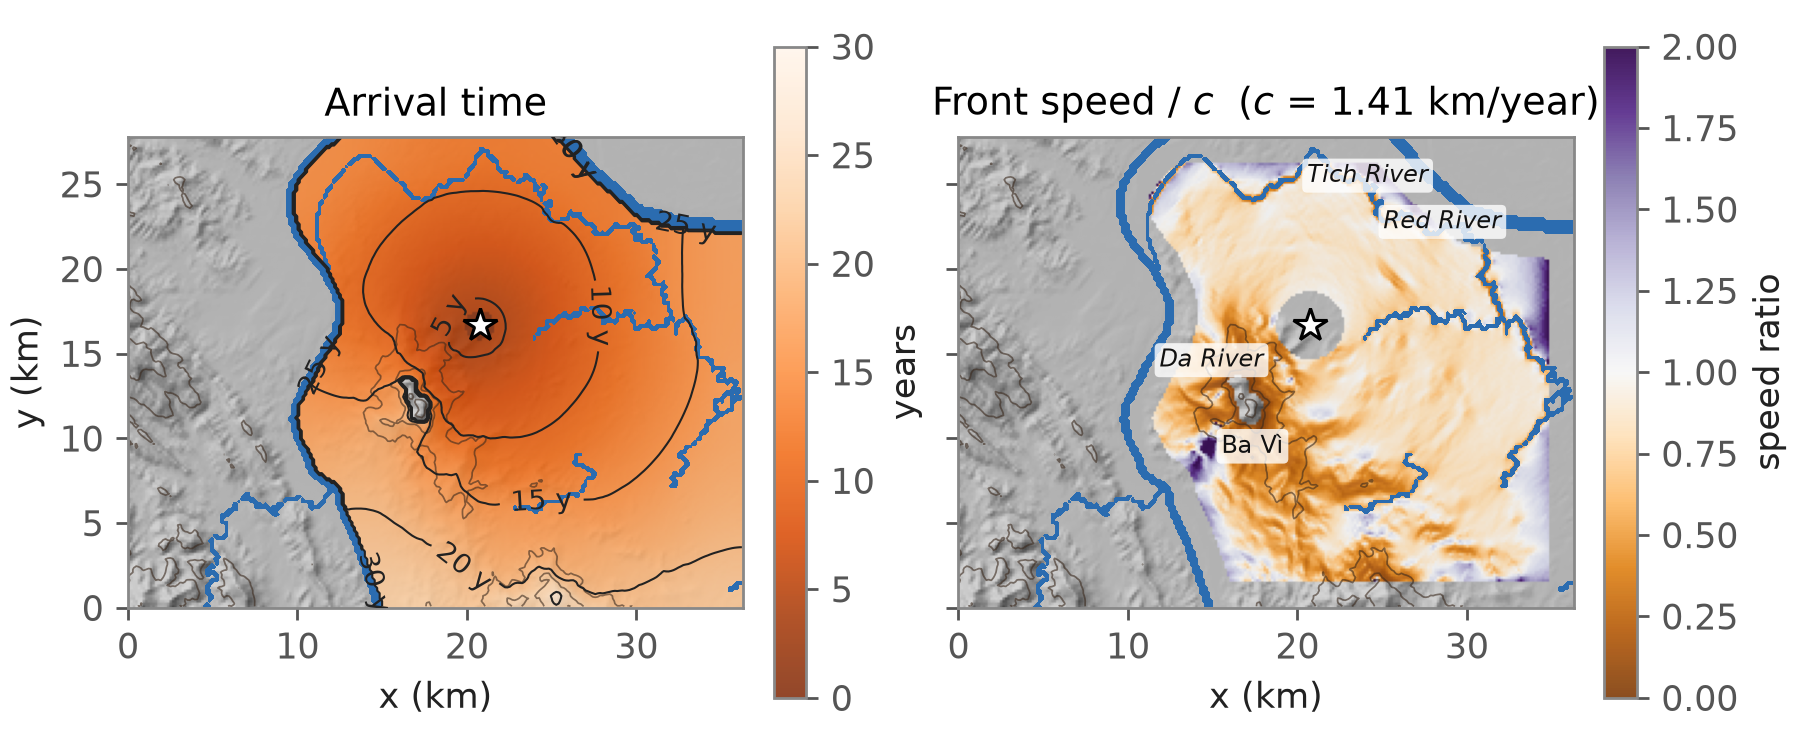
\includegraphics[width=\textwidth]{./FigB3_bavi_arrival_speed.png}
      \end{center}
      \begin{block}{Front speed $= 1/|\nabla T_{\mathrm{arrival}}|$}
          Orange: the front slows down. Purple spots: two fronts meet (not a real acceleration). Not reached after 30 years: $36\%$ of the land.
      \end{block}
    \end{frame}

    \begin{frame}{5. Results and Discussion}{Real Terrain (Ba V\`{\i}): Results}
      \begin{center}
        \small
        \renewcommand{\arraystretch}{1.3}
        \begin{tabular}{l l l}
          \hline
          \textbf{Effect} & \textbf{Where} & \textbf{Result} \\
          \hline
          Normal spreading & flat plains ($s < 0.05$) & front speed $\approx 0.88\,c$ (median) \\
          Slowed down & steep slopes ($s > 0.3$) & front speed $\approx 0.35\,c$ (median) \\
          Slightly slowed & Tich River & crossed \\
          Blocked & Da River, Red River & far banks empty after 30 years \\
          Not colonized & Ba V\`{\i} summit & $K \approx 4 < 20$ \\
          \hline
        \end{tabular}
      \end{center}
      \begin{block}{Result}
          After $30$ years the population occupies $64\%$ of the land: the far banks of the big rivers and the summit stay empty.
      \end{block}
    \end{frame}

  \subsection{Case Study: Neolithic Europe}
    \begin{frame}{5. Results and Discussion}{Case Study: Spread of Farming into Europe}
      \begin{block}{Published study \hfill [14]}
          R. Pinhasi, J. Fort, A. J. Ammerman, ``Tracing the Origin and Spread of Agriculture in Europe,'' \textit{PLoS Biology} 3(12): e410, 2005 (open access, data in Table S1).
      \end{block}
      \begin{block}{Question}
          Farming spread from the Near East into Europe. How fast did the farming front move, and can a reaction--diffusion model predict this speed?
      \end{block}
      \begin{block}{Data and method}
          \begin{itemize}
            \item $735$ early Neolithic sites in Europe, Anatolia and the Near East, each with its earliest radiocarbon date: from $10\,890$ to $4\,500$ years BP.
            \item Distance of every site from the probable origin, Abu Madi (Sinai).
            \item Linear regression of distance against date $\Rightarrow$ speed of the front.
          \end{itemize}
      \end{block}
    \end{frame}

    \begin{frame}{5. Results and Discussion}{Case Study: the Data}
      \begin{center}
        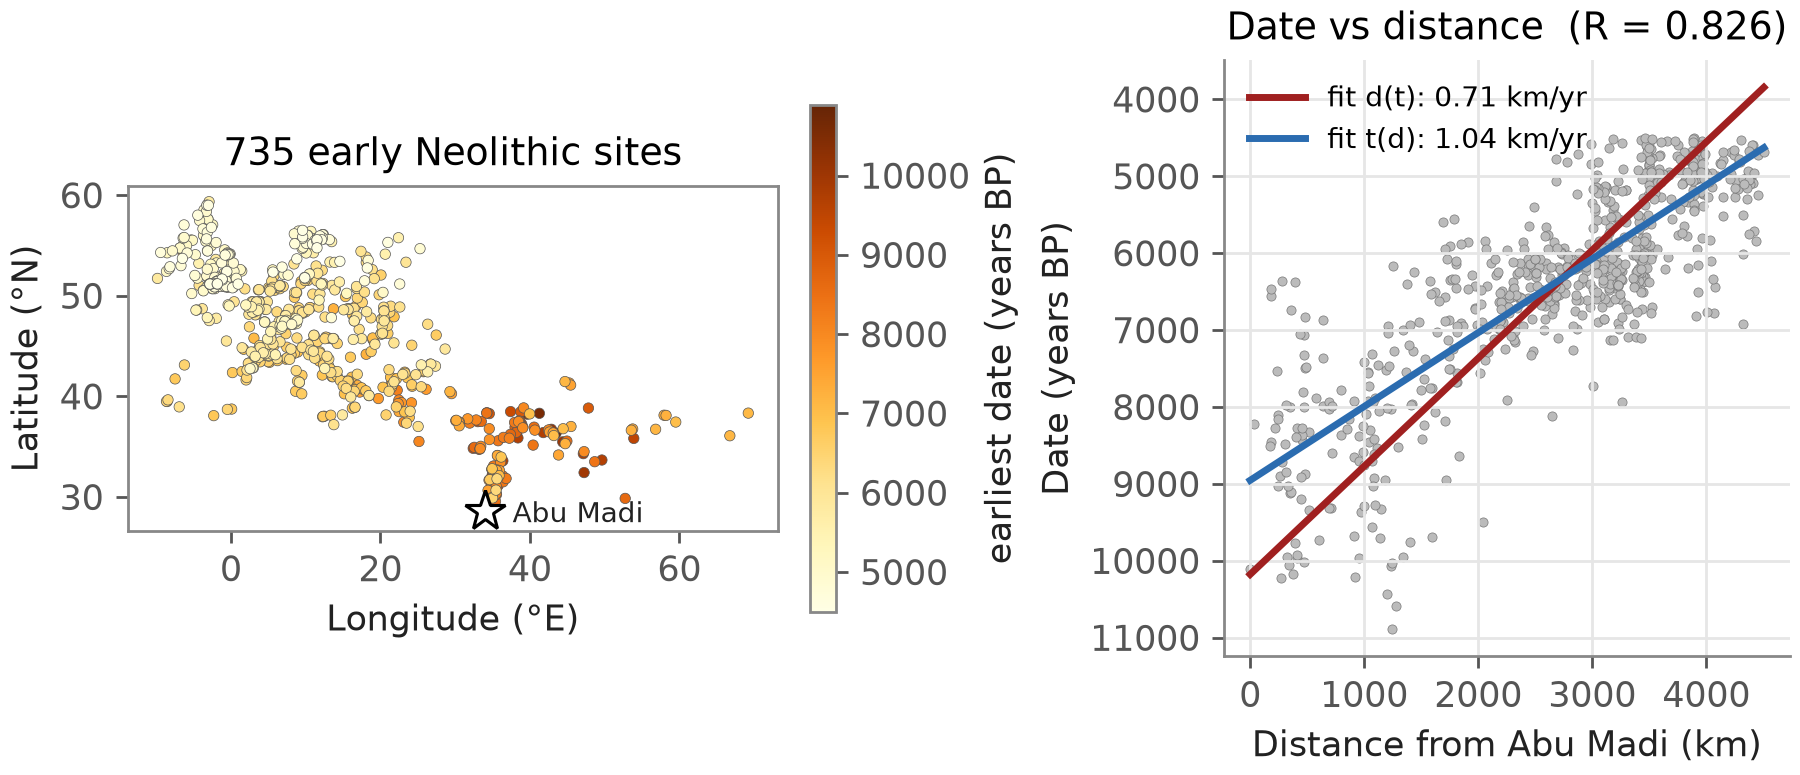
\includegraphics[width=\textwidth]{./FigN1_neolithic_data.png}
      \end{center}
      \begin{block}{Our refit of the published data}
          $R = 0.826$; front speed $0.71$--$1.04$ km/year from the two regressions \\
          (paper: $R = 0.827$, \; $0.71 \pm 0.04$ and $1.04 \pm 0.05$ km/year).
      \end{block}
    \end{frame}

    \begin{frame}{5. Results and Discussion}{Case Study: Model and Parameters}
      \begin{block}{Fisher--KPP speed, without and with a generation time $T$ \hfill [14], [15]}
          $$
          v_{\mathrm{Fisher}} = 2\sqrt{aD},
          \qquad
          v_{\mathrm{delay}} = \frac{2\sqrt{aD}}{1 + aT/2},
          \qquad
          D = \frac{m}{4T}
          $$
      \end{block}
      \begin{center}
        \small
        \renewcommand{\arraystretch}{1.25}
        \begin{tabular}{l l l}
          \hline
          \textbf{Parameter} & \textbf{Value (from the paper)} & \textbf{Meaning} \\
          \hline
          $a$ & $0.029$--$0.035$ /year & initial growth rate of farmers \\
          $m$ & $900$--$2200$ km$^2$ & mobility (per generation) \\
          $T$ & $29$--$35$ years & generation time \\
          $D = m/4T$ & $6.4$--$19.0$ km$^2$/year & diffusion coefficient \\
          \hline
          $v_{\mathrm{Fisher}}$ & $0.86$--$1.63$ km/year & classic Fisher--KPP \\
          $v_{\mathrm{delay}}$ & $0.57$--$1.08$ km/year & time-delayed Fisher \\
          \hline
        \end{tabular}
      \end{center}
    \end{frame}

    \begin{frame}{5. Results and Discussion}{Case Study: Model vs Data}
      \begin{center}
        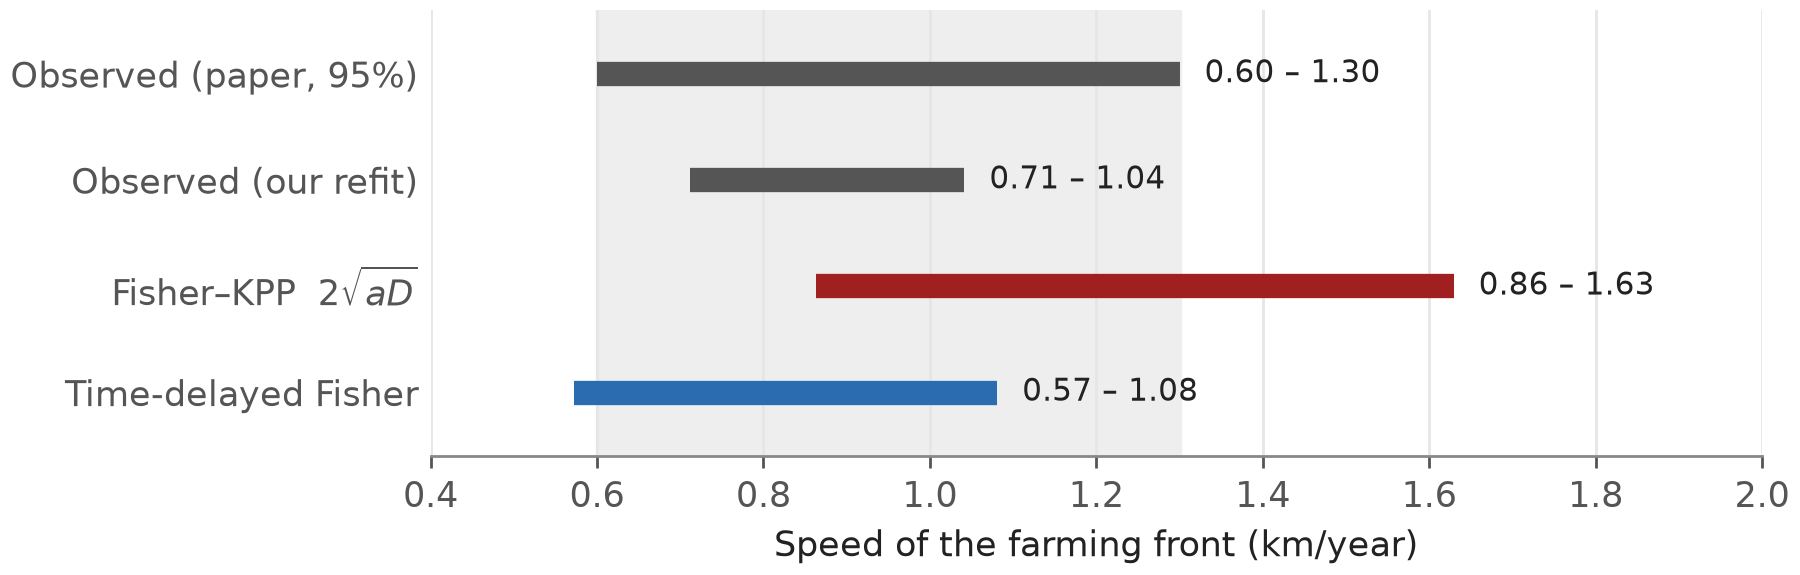
\includegraphics[width=\textwidth]{./FigN2_neolithic_speed.png}
      \end{center}
      \begin{block}{Result}
          The Fisher--KPP speed has the right order of magnitude ($\sim 1$ km/year) but is partly too fast. With the generation time, the predicted $0.57$--$1.08$ km/year lies inside the observed $0.6$--$1.3$ km/year: farming spread with moving farmers, as a reaction--diffusion front.
      \end{block}
    \end{frame}

  \subsection{Comparison of Methods}
    \begin{frame}{5. Results and Discussion}{Comparison of FDM and FEM}
      \begin{center}
        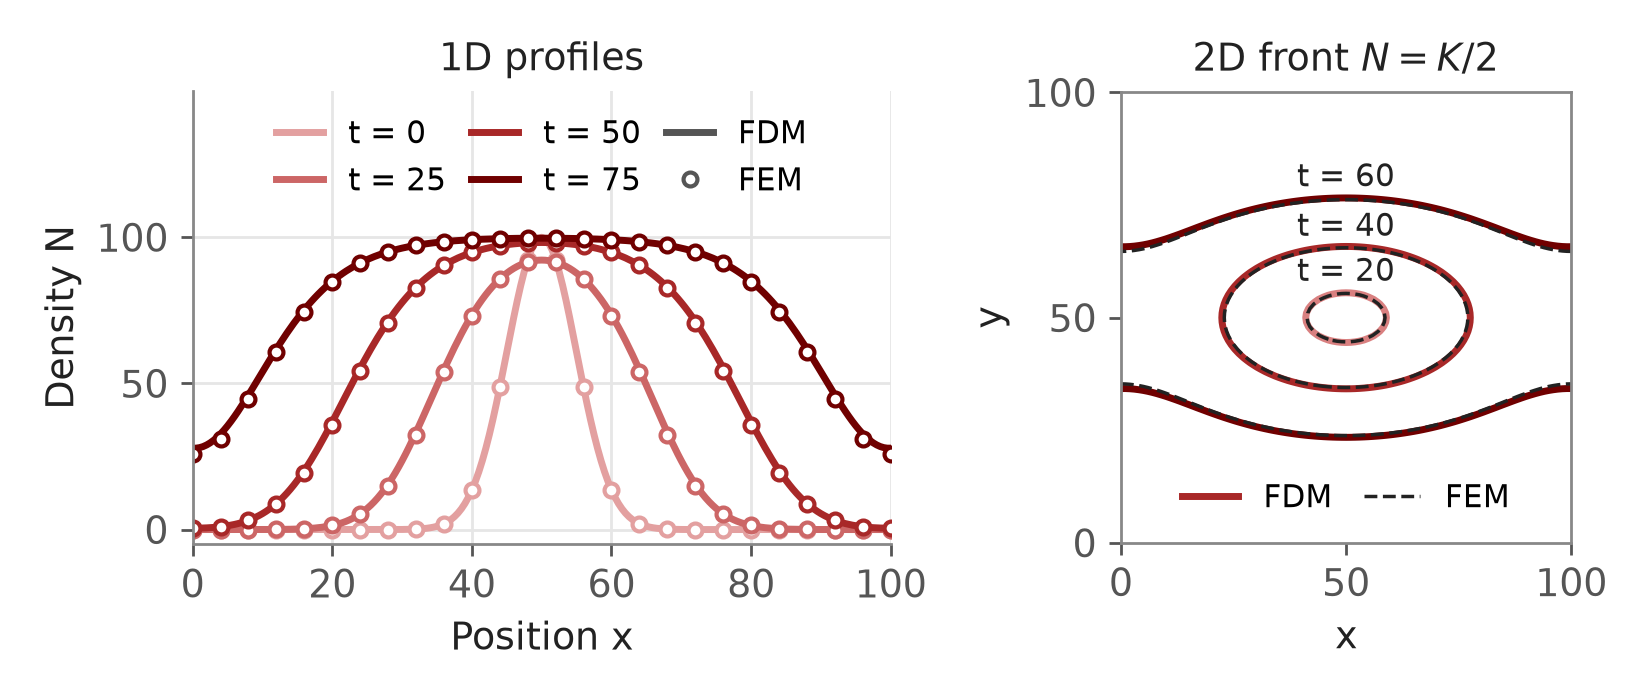
\includegraphics[width=\textwidth]{./Fig5_fem_vs_fdm.png}
      \end{center}
      \begin{block}{Result}
          With a time step $6$--$10\times$ larger, FEM stays within $3\%$ of $K$ of the FDM solution (max difference: $2.2\%$ in 1D, $2.6\%$ in 2D).
      \end{block}
    \end{frame}

    \begin{frame}{5. Results and Discussion}{Explicit Euler vs ADI (2D, $t = 60$)}
      \begin{center}
        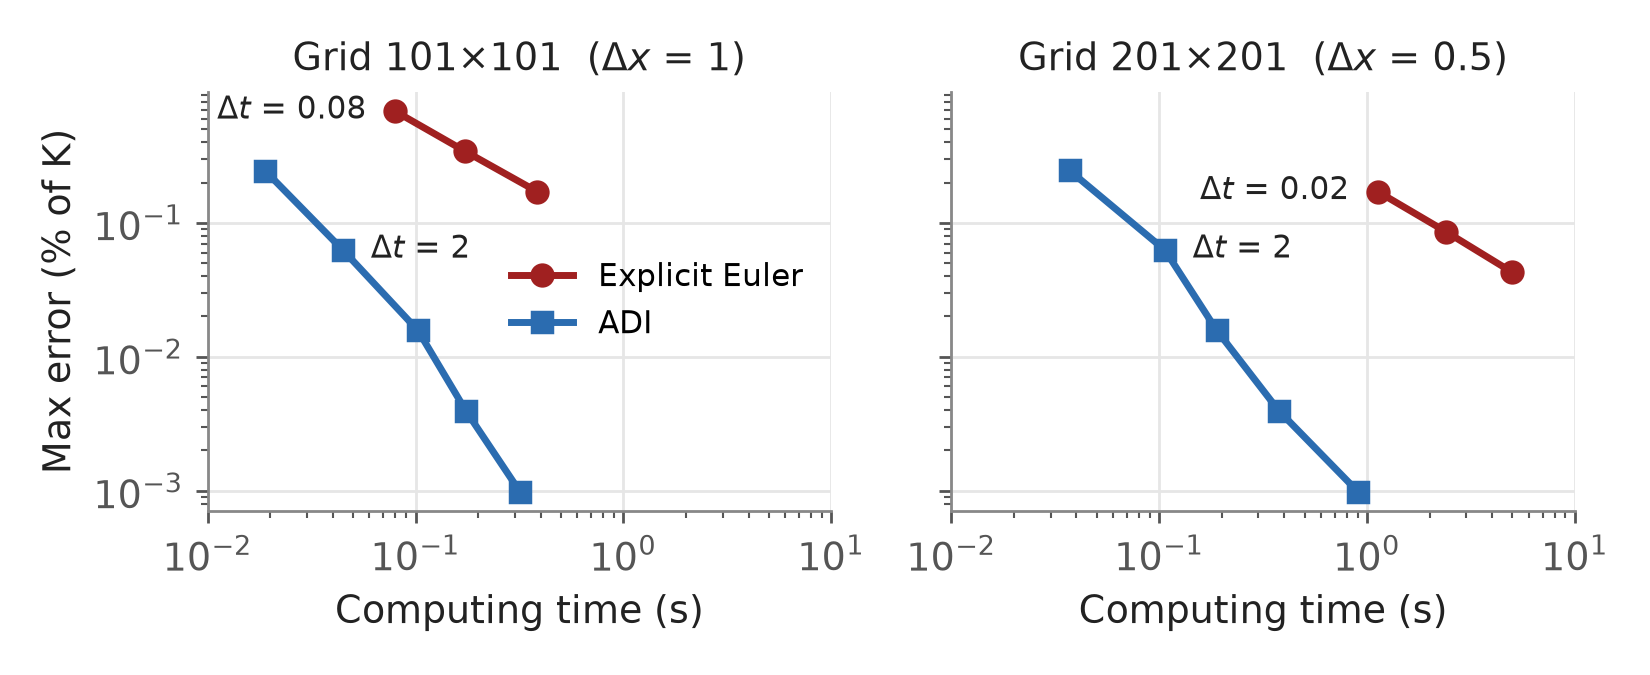
\includegraphics[width=0.92\textwidth]{./Fig6_adi_benchmark.png}
      \end{center}
      \begin{block}{Result}
          Grid $201\times201$: ADI ($\Delta t = 2$) is $\approx 10\times$ faster and $3\times$ more accurate than explicit Euler ($\Delta t = 0.02$).\\
          Halving $\Delta x$: explicit Euler $\approx 13\times$ slower, ADI only $\approx 2.5\times$.
      \end{block}
    \end{frame}

  \subsection{Discussion}
    \begin{frame}{5. Results and Discussion}{Discussion}
      \begin{block}{What the results show}
          \begin{itemize}
            \item \textbf{Homogeneous habitat:} the population forms a front that moves at an almost constant speed, close to $c = 2\sqrt{rD}$.
            \item \textbf{Real terrain (Ba V\`{\i}):} slopes slow the front ($\approx 0.35\,c$), wide rivers stop it, the poor habitat of the summit is never colonized.
            \item \textbf{Real data (Neolithic Europe):} the Fisher--KPP speed has the right order of magnitude; a generation time brings it inside the observed range.
            \item \textbf{Numerics:} FDM, FEM and ADI agree; FEM and ADI allow much larger time steps.
          \end{itemize}
      \end{block}
      \begin{block}{Limitations}
          \begin{itemize}
            \item The Ba V\`{\i} parameters are illustrative, not fitted to a species.
            \item Deterministic model: no randomness, no long jumps, no bridges or roads.
            \item $D$, $r$, $K$ do not change in time (no seasons, no climate change).
          \end{itemize}
      \end{block}
    \end{frame}

\section{Conclusion}
    \begin{frame}{6. Conclusion}
      \begin{block}{Conclusion}
          \begin{itemize}
              \item We extended the Logistic Growth Model from an ODE to a Reaction-Diffusion PDE to describe spatial population dynamics.
              
              \item The model captures both population growth and spatial diffusion.
              
              \item Numerical simulations illustrate how the population spreads and approaches the carrying capacity over time.
              
              \item Different diffusion coefficients can produce different spatial spreading patterns.
          \end{itemize}
      \end{block}
    \end{frame}

\section{References}
  \begin{frame}[allowframebreaks]{References}
    \begin{itemize}
        \item[\textbf{[1]}] J. D. Murray,
        \textit{Mathematical Biology I: An Introduction},
        3rd ed., Springer, 2002.

        \item[\textbf{[2]}] R. A. Fisher,
        ``The Wave of Advance of Advantageous Genes,''
        \textit{Annals of Eugenics}, vol. 7, pp. 355--369, 1937.

        \item[\textbf{[3]}] A. N. Kolmogorov, I. G. Petrovskii, and N. S. Piskunov,
        ``A Study of the Equation of Diffusion with Increase in the Quantity of Matter,
        and Its Application to a Biological Problem,''
        \textit{Moscow University Mathematics Bulletin}, 1937.

        \item[\textbf{[4]}] R. J. LeVeque,
        \textit{Finite Difference Methods for Ordinary and Partial Differential Equations},
        SIAM, 2007.

        \item[\textbf{[5]}] J. G. Skellam,
        ``Random Dispersal in Theoretical Populations,''
        \textit{Biometrika}, vol. 38, pp. 196--218, 1951.

        \item[\textbf{[6]}] D. A. Andow, P. M. Kareiva, S. A. Levin, and A. Okubo,
        ``Spread of Invading Organisms,''
        \textit{Landscape Ecology}, vol. 4, pp. 177--188, 1990.

        \item[\textbf{[7]}] J. D. Murray, E. A. Stanley, and D. L. Brown,
        ``On the Spatial Spread of Rabies among Foxes,''
        \textit{Proc. R. Soc. Lond. B}, vol. 229, pp. 111--150, 1986.

        \item[\textbf{[8]}] K. R. Swanson, E. C. Alvord Jr., and J. D. Murray,
        ``A Quantitative Model for Differential Motility of Gliomas in Grey and White Matter,''
        \textit{Cell Proliferation}, vol. 33, pp. 317--329, 2000.

        \item[\textbf{[9]}] A. J. Ammerman and L. L. Cavalli-Sforza,
        \textit{The Neolithic Transition and the Genetics of Populations in Europe},
        Princeton University Press, 1984.

        \item[\textbf{[10]}] A. Giometto, A. Rinaldo, F. Carrara, and F. Altermatt,
        ``Emerging Predictable Features of Replicated Biological Invasion Fronts,''
        \textit{PNAS}, vol. 111, pp. 297--301, 2014.

        \item[\textbf{[11]}] M. G. Larson and F. Bengzon,
        \textit{The Finite Element Method: Theory, Implementation, and Applications},
        Springer, 2013.

        \item[\textbf{[12]}] D. W. Peaceman and H. H. Rachford Jr.,
        ``The Numerical Solution of Parabolic and Elliptic Differential Equations,''
        \textit{Journal of the SIAM}, vol. 3, pp. 28--41, 1955.

        \item[\textbf{[13]}] G. Strang,
        ``On the Construction and Comparison of Difference Schemes,''
        \textit{SIAM Journal on Numerical Analysis}, vol. 5, pp. 506--517, 1968.

        \item[\textbf{[14]}] R. Pinhasi, J. Fort, and A. J. Ammerman,
        ``Tracing the Origin and Spread of Agriculture in Europe,''
        \textit{PLoS Biology}, vol. 3, no. 12, e410, 2005.

        \item[\textbf{[15]}] J. Fort and V. M\'endez,
        ``Time-Delayed Theory of the Neolithic Transition in Europe,''
        \textit{Physical Review Letters}, vol. 82, pp. 867--870, 1999.
    \end{itemize}
  \end{frame}


\section*{Acknowledgement}
    \begin{frame}[plain]
      \begin{center}
          \vspace{1.2cm}
          {\usebeamerfont{title}
          \textcolor{myNewColorA}{\Huge\textbf{Thank You!}}
          }
          \vspace{0.4cm}
          {\Large
          \textcolor{myNewColorB}{Questions \& Discussion}
          }
          \vspace{0.7cm}
          \textcolor{myNewColorC}{\rule{0.55\textwidth}{1.2pt}}
          \vspace{0.5cm}

          {\normalsize
          \textbf{Summer Program on Mathematical Modeling 2026}
          }
          \vspace{0.2cm}

          {\small
          Modeling Spatial Population Growth Using Reaction-Diffusion PDEs
          }
          \vspace{0.6cm}

          {\small
          Tran Dang Quang Minh\\
          VNU Hanoi University of Science
          }
          \vfill
          
\includegraphics[height=0.7cm]{./HUS.png}
          \hspace{0.3cm}
          
\includegraphics[height=0.7cm]{./NWU.png}
      \end{center}
    \end{frame}

\end{document}
